\subsection{Разработка даталогической и физической моделей базы данных}
\label{sec:design:db}

Как было упомянуто ранее, в программном средстве, описываемом данным дипломным проектом, будет использоваться
СУБД PostgreSQL. Описание схемы БД для нее может производится в том числе с помощью механизма миграций и моделей в веб-фреймворке
Ruby on Rails. Тем не менее, разрабатывать модель схемы можно с помощью любых средств, однако затем разработанную 
модель нужно вручную перевести в формат, используемый СУБД. 

На даталогическом уровне модель предметной области представляется в привязке к конкретной СУБД и описывает способ
организации данных безотносительно их физического размещения. Описывать модель можно с помощью специальных
графических нотаций~\cite{kulikov_db_workbook}. 

Модель даталогического уровня разработаем на основании инфологической модели, описание которой приведено в
пункте \ref{sec:domain:model:db}. 

СУБД PostgreSQL не просто реляционная, а объектно-реляционная \linebreak СУБД. Это даёт ему некоторые преимущества над другими SQL
базами данных с открытым исходным кодом, такими как MySQL, MariaDB и Firebird.

Фундаментальная характеристика объектно-реляционной базы данных — это поддержка пользовательских объектов и их
поведения, включая типы данных, функции, операции, домены и индексы. Это делает PostgreSQL невероятно гибким и надежным.
Среди прочего, он умеет создавать, хранить и извлекать сложные структуры данных.

Существует обширный список типов данных, которые поддерживает PostgreSQL. Кроме числовых, с плавающей точкой, текстовых,
булевых и других ожидаемых типов данных (а также множества их вариаций),\linebreak PostgreSQL может похвастаться поддержкой uuid,
денежного, перечисляемого, геометрического, бинарного типов, сетевых адресов, битовых строк, текстового поиска, xml,
json, массивов, композитных типов и диапазонов, а также некоторых внутренних типов для идентификации объектов и
местоположения логов. Справедливости ради стоит сказать, что MySQL, MariaDB и Firebird тоже имеют некоторые из этих
типов данных, но только PostgreSQL поддерживает их все.

Поддержка JSON в PostgreSQL позволяет перейти к хранению schema-less данных в SQL базе данных. Это может быть полезно,
когда структура данных требует определённой гибкости: например, если в процессе разработки структура всё ещё меняется
или неизвестно, какие поля будет содержать объект данных.

Тип данных JSON обеспечивает проверку корректности JSON, который позволяет использовать специализированные JSON
операторы и функции, встроенные в Постгрес для выполнения запросов и манипулирования данными. Также доступен тип
JSONB — двоичная разновидность формата JSON, у которой пробелы удаляются, сортировка объектов не сохраняется, вместо
этого они хранятся наиболее оптимальным образом, и сохраняется только последнее значение для ключей-дубликатов.
JSONB обычно является предпочтительным форматом, поскольку требует меньше места для объектов, может быть
проиндексирован и обрабатывается быстрее, так как не требует повторного синтаксического анализа. 

Для создания даталогической модели базы данных, используемой в разрабатываемом приложении будем использовать расширение
диаграммы классов UML 2.1, предназначенное для моделирования баз данных. Полученная диаграмма, представленная на
рисунке~\ref{fig:design:db:model}, будет являться моделью базы данных даталогического уровня.

Физический уровень моделирования БД описывает конкретные таблицы, связи, индексы, методы хранения, настройки
производительности, безопасности. Описывать модель можно с помощью средств, уместных для предметной
области~\cite{kulikov_db_workbook}.

Индексы -- это специальные структуры, применяемые для ускорения операций взаимодействия с данными.
Целесообразно реализовать следующие индексы:

\begin{itemize}
	\item по названиям проектов, позиций, департаментов, навыков;
	\item по электронной почте и имени пользователей.
\end{itemize}

Для идентификации используется специальное поле id, которое внедряется во все сущности.

Остальные настройки будут применяться непосредственно при развертывании программной системы, поэтому в данном разделе
не\linebreakрассматриваются.

\begin{figure}[!ht]
	\centering
	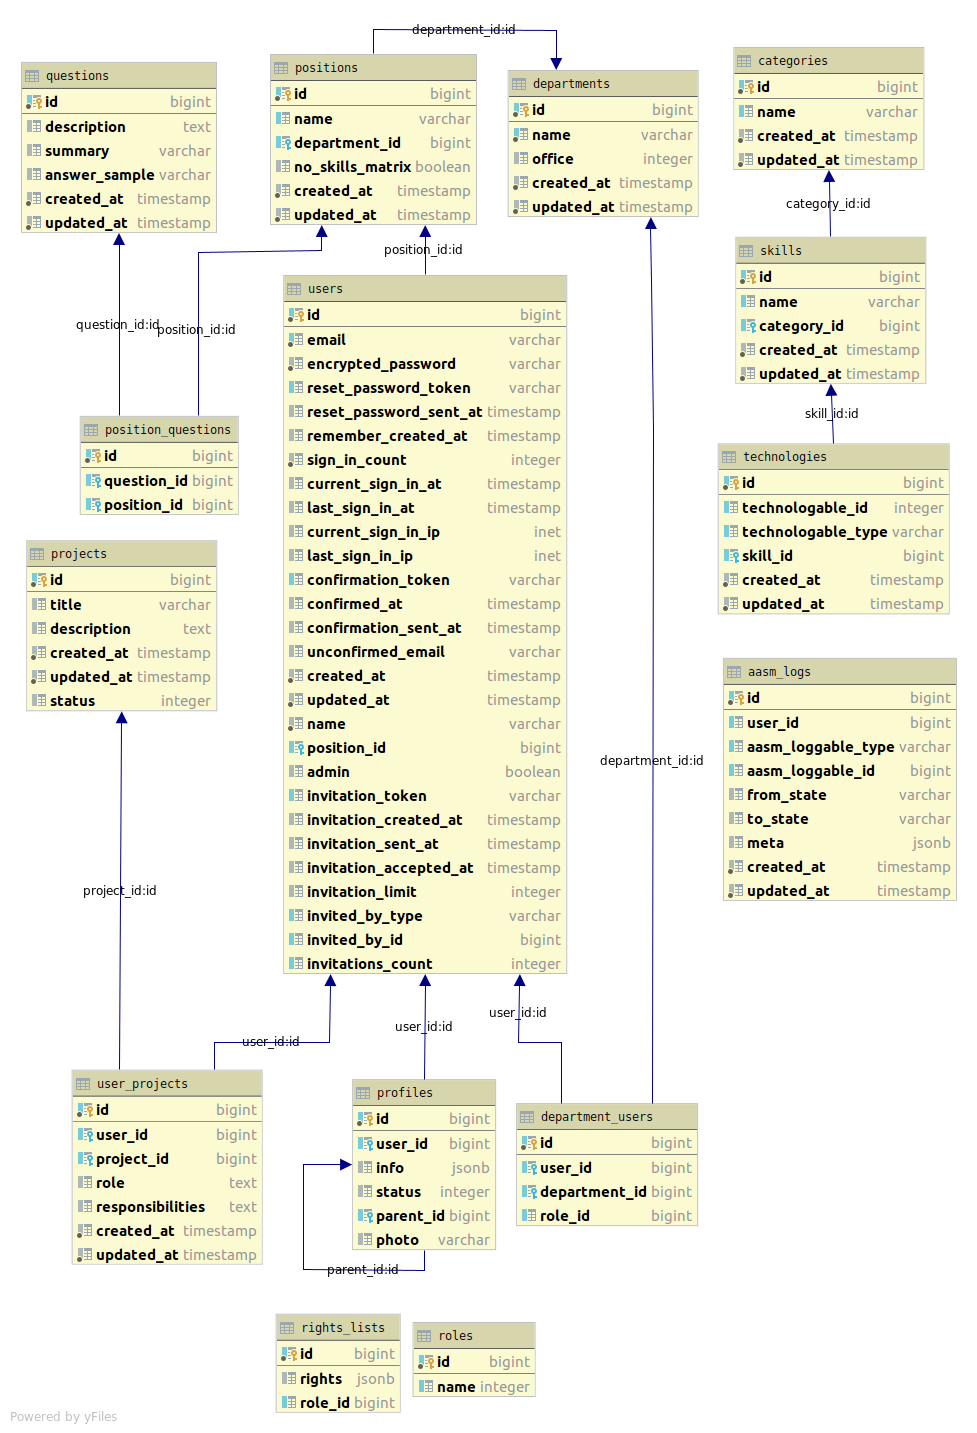
\includegraphics[scale=0.47]{database.png} 
	\caption{Даталогическкая модель базы данных программного средства}
	\label{fig:design:db:model}
\end{figure}
